\marcos{Related work chapter: here are the broad areas (paint the big picture). Maybe even a real picture, a figure that shows the different areas. A conceptual model of how to navigate the litterature, a map of sorts. Here are some representative works, here is how you should think about them. There will be some references, details in the related works. focus on data abstraction (map generalization, also cover some other stuff), less focus on data serving (database, key-value stores, caching, CDN, etc.).}

\pitfall{\emph{I Am So Unique:} Do not ignore previous work when writing up your paper. You have to convince the reader that you have done something new, and the only way to do that is to explain how it is different than what has already been done. All research takes place in some kind of intellectual context, and your job as author is to situate what you have done within a framework of that context. A good previous work section is a mini-taxonomy of its own, where you decide on meaningful categorization given your specific topic. Proposing new names for old techniques or ideas may sneak your work past some reviewers, but will infuriate those who know of that previous work. This tactic will also make you lose credibility with knowledgeable readers. If you cannot find anything related to what you have done, it?s more likely that you?re looking in the wrong subfield than that your work is a breakthrough of such magnitude that there is no context. Remember to discuss not only work that has been done on similar problems to your own, but also work that uses similar solutions to yours that occurs in different problem domains. This advice is even more critical if you were lax about doing a literature review before you started your project. If you find work similar to your own, you have a fighting chance of carefully differentiating yours in the writeup, but if a reviewer is the one to
bring it to your attention, the paper is most likely dead.}

\pitfall{\emph{Enumeration Without Justification:} Simply citing the previous work is necessary but not sufficient. A description that 'X did Y', even if it includes detail, is not enough. You must explain why this previous work does not itself solve your problem, and what specific limitations of that previous work your approach does address. Every paper you cite in the previous work section is a fundamental challenge to the very existence of your project. Your job is to convince a skeptical reader that the world needs your new thing because it is somehow better than a particular old thing. Moreover, it's not even enough to just make the case that yours is different: yours must be better. The claims you make must, of course, be backed up by your validation in a subsequent results section.

A good way to approach the previous work section is that you want to tell to a story to the reader. Figure out the messages you want to get across to the reader, in what order, and then use the references to help you tell this story. It is possible to group the previous work into categories, and to usefully discuss the limitations of the entire category.}



%\begin{quote}
%Wherever there is life, there is twist and mess: the frizz of an arctic lichen, the tangle of brush along a bank, the dogleg of a dog's leg, the way a line has got to curve, split or knob. The planet is characterised by its very jaggedness, its random heaps of mountains, its frayed fringes of shore... Think of a contour globe, whose mountain ranges cast shadows, whose continents rise in bas-relief above the oceans. But then: think of how it really is. These heights aren't just suggested; they're there... What if you had an enormous globe in relief that was so huge it showed roads and houses -- a geological survey globe, a quarter of a mile to an inch -- of the whole world, and the ocean floor! Looking at it, you would know what had to be left out: the free-standing sculptural arrangement of furniture in rooms, the jumble of broken rocks in a creek bed, tools in a box, labyrinthine ocean liners, the shape of snapdragons, walrus... The relief globe couldn't begin to show trees, between whose overlapping boughs birds raise broods, or the furrows in bark, where whole creatures, creatures easily visible, live out their lives and call it world enough.' (Dillard 1974: 141 -- 3) -- reproduced from Weibel~\cite{weibel1999generalising}
%\end{quote}

%wilkinson2006grammar....

% Properly designed data visualizations enable people to see the big picture of otherwise unfathomable phenomena, such government spending~\cite{mytimes:obama:budget}, the geography of the Earth~\cite{google:maps}, and complex aspects of human history~\cite{foo} and culture~\cite{vocab}. 
% http://www.theguardian.com/news/datablog/ng-interactive/2014/may/07/sunrise-twitter-animated-map
% http://rappers.mdaniels.com.s3-website-us-east-1.amazonaws.com/
% http://www.nytimes.com/interactive/2012/02/13/us/politics/2013-budget-proposal-graphic.html

%\emph{Geographic information represents our understanding of the association of phenomena with their location on and near the Earth's surface. When presented in map form, an essential aspect of that information is that it may be adapted in semantic abstraction and level of geometric detail according to the purpose of the map and the extent of the Earth that is being considered at any one time. Representations of small areas in detail result in so-called large-scale maps, while representations of large regions in lesser detail are referred to as small-scale maps. Traditionally cartographers have performed the task of adapting the content and the level of detail of a map to suit its scale and purpose and this process is called map generalisation.}

% What is map visualization and why is it an interesting problem?

% \marcos{Regarding the chapters for the three papers: review the text, see if there are any arguments that can be improved; no time to redo non-text work.}
% \todo{Cite everything that is cited by The Case for Data Visualization Management Systems (33 citations)}


%This dissertation focuses on multi-scale selection and projection of points for geographical mash-ups, in particular points that are stored in relational tables. The motivations are: (1) most frequently, data for visualizations is stored in a relational database management system (RDBMS)~\cite{wu2014case}, (2) the process of selection and projection retains the identity of individual records in a map, which allows for user interaction. In contrast, aggregation trades interactivity for statistical information, (3) high-quality background maps are available, which leaves the simpler problem of 


%Map visualization studies how to visually represent the geography of the Earth at multiple scales (i.e. with pan and zoom) on restricted mediums, such as computer screens. Map visualization is a facet of the data visualization field, which is the study and creation of (interactive) visual representations of data to reinforce human cognition~\cite{friendly2008milestones}. However, the specific value proposition of geographical maps is clear: maps save lives~\cite{openstreetmap2010haiti}; maps crucially assist navigation~\cite{something}; maps increase the transparency and efficiency of our societies~\cite{gst2012friedata}. The human human mind has such a strong affinity for spatial reasoning that map metaphors are used to reason even about non-spatial phenomena~\cite{shahaf2013informationcartography, daniels2014vocabulary}.

%More and more, organizations with no strong tradition for geography (e.g. news agencies) communicate spatial narratives using maps~\cite{nytimes2010iraq}. As a consequence, more and more professionals will need to acquire the skills to craft map visualizations. One of the most crucial problems in map creation is the mismatch between data volume and the small representational budget of computer screens. For example, a laptop display (e.g. 2880 x 1800 pixels) can display just a few thousand symbols without overlap, which is entirely indadequate for displaying most geographical datasets. Necessarily, geographical data must be abstracted (e.g. filtered~\cite{} or aggregated~\cite{}) according to scale in order to produce a legible and useful map. However, filtering and aggregation for maps is much more complex than the similarly named operations in statistics. Within map visualization, the disciplin of map generalization studies how geographical data should be abstracted as the scale changes. In contrast to selection, projection and aggregation in the relation algebra, map generalization must select, project and aggregate data \emph{holistically} according to visual constraints and objectives~\cite{weibel1999generalising}.

% Why GIS is inadequate
%Traditionally, maps have been crafted by experts in Geographical Information Systems (GIS). However, a new situation exists on the web today that significantly marginalizes the use for traditional GIS. First, the demand for multi-scale maps on the web is rising faster than the number of GIS experts who know how to craft them (using traditional GIS); therefore, map visualizations must be \emph{expressible by non-experts}. Second, web maps that run on top of cloud infrastructures can now integrate huge datasets (billions of data items); therefore, map visualization systems must be \emph{scalable in the size of data}. Third, web maps today can quickly reach millions of users who can interact with map visualization 24 x 7 using mobile devices; therefore, map visualization systems must be \emph{scalable in the number of concurrent users} and \emph{highly available}. In short, GIS was not designed to satisfy these requirements, which merits the study of a new category of systems.


%\emph{copy-pasted} While data can be both numerical and non-numerical, this thesis will focus on geographical data that is stored in tables, e.g. rows in an RDBMS. At first, this may seem constricted, however tables are versatile and make up the bulk of all data that is visualized today~\cite{wu2014case}.


%\emph{What are the requirements?}

%\emph{What is special about geography?}

% Requirements for new system: MVMS

% MOVE TO RELATED WORK
%Data Visualization Management Systems (DVMS) have been proposed as a solution for data-driven visualizations on the web today~\cite{wu2014case, fekete2012dmvis}. The API of a fully-fledged DVMS includes components for both data management, visualization design, and visualization sharing~\cite{foo}. A DVMS must be scalable both in the size of data~\cite{lins2013nanocubes, Im2013visreduce, battle2013scalar, liu2013immens} and audience~\cite{viegas2007manyeyes}. Additionally, it is crucial that designers can craft visualizations using an interface that is both intuitive, efficient (in terms of wall-clock time) and expressive. In the geographical domain, prototypes of such systems include Google Fusion Tables~\cite{google2014fusiontables}, and CartoDB~\cite{cartodb2014cartodb}. To make the distinction clear, this dissertation will introduce the term Map Visualization Management Systems (MVMS) and use it to refer to for DVMS that are specialized for map visualization.

%One of the most popular types of map visualizaitons is the geospatial mashup. Mash-ups are popular because they combine something we know, such as a high-quality background map, with something we would like to find out, such as a new and exciting thematic overlay. Thanks to an active eco-system of data enthusiasts, thematic overlays now cover the full spectrum of human interests, such as culture~\cite{foo}, nature~\cite{foo}, war~\cite{wikileaks}, and peace~\cite{unstats}. In the ``always on'' world of mobile devices, millions of users can access an online map 24 x 7. For this reason, maps are a crucial form of communication that is used by international organizations~\cite{un}, news agencies~\cite{guardian}, and amateurs alike~\cite{shiplogs}.

%\emph{How has the world changed; what is the new situation?} The web today is home to an open eco-system of data providers and data consumers who create and combine a huge diversity of curated~\cite{gst2014digitalmapsupply} and user-contributed~\cite{wikipedia} datasets. In combination, open data covers the full spectrum of human interests, including culture~\cite{rapgenius}, economics~\cite{worldbank}, geography~\cite{gst2014digitalmapsupply}, demography~\cite{unstats} and politics~\cite{data:gov}. Indeed, the value proposition of open data is clear: it increases the level of transparency, efficiency and enlightenment in our societies~\cite{hans:rosling, offentlige:data:i:spil}. Consequently, the availability of open data has created a great demand for online data-driven visualizations, e.g. maps~\cite{mapref}, bubbles~\cite{datavizref}, and buckets~\cite{datavizref}. Since data visualizations are so useful they are often shared online, for example on social media, where they can quickly attract an audience of millions~\cite{nytimes2012obamabudget, guardian2012wikileaks}. 


%\note{Challenges are: (1) the man-hours required for expressing data visualization, (2) the scalability of data processing for visualization, (3) the cost of data distribution, e.g. CDN}

%\todo{Revisit this section when Related Works is done. Remember to read all relevant papers}

%\todo{Rehash arguments from: The Case for Visualization Management Systems~\cite{wu2014case}: % http://www.vldb.org/pvldb/vol7/p903-wu.pdf
%\begin{itemize}
%\item The case for an integrated Data Visualization Management System (DVMS).
%\item Data today is mostly stored in RDBMS
%\item Visualizations today retrieve data from a database and render it externally
%\item Decoupled approach results in significant duplication of functionality, such as aggregation and filters, and misses tremendous opportunities for cross-layer optimizations
%\item Declarative visualisation languages that fully compiles the end-to-end visualisation pipeline into relational algebra queries
%\item Thus, DVMS are expressive via the language and performant via traditional and visualisation specific optimizations to scale interactive visualizations to massive datasets.
%\end{itemize}
%Managing Data for Visual Analytics: Opportunities and Challenges~\cite{fekete2012dmvis}: 
%Visual Analytics: Definition, Process and Challenges: % https://hal.archives-ouvertes.fr/file/index/docid/272779/filename/VAChapter_final.pdf
}

%\todo{Investigate also these papers: Visual Exploration of Big Spatio-Temporal Urban Data: A Study of New York City Taxi Trips~\cite{ferreira2013newyork}, Visual Analytics Infrastructures: From Data Management to Exploration~\cite{fekete2013visual}, Dive in!: enabling progressive loading for real-time navigation of data visualizations~\cite{glueck2014dive}.}





First, designers of data visualizations must address the crucial problem of expressing appropriate data abstractions for multi-scale , i.e. appropriate selection or aggragation of the data to be presented. Otherwise, the finite resources available for visual representation of the data will be quickly depleted as the data grows in size~\cite{topfer:selection, weibel, stonebraker}. For example, a computer screen only has a finite set of pixels that can be used to graphically represent the data. Furthermore, a data visualization has to be legible, representative and possibly multi-scale. For example, a digital map, which is a visualization of geographical data, must allow users to zoom in and out to expore the Earth at different granularities. Consequently, the data must be coherently abstracted in a way that satisfies multiple requirements. In general, designers cannot manually perform data abstraction over large datasets, because this would be too time consuming. Therefore, the data abstraction process must be at least partially automated. However, automation implies loss of control. How can designers remain in control of a partially automated data abstraction process, such that a desirable result is obtained, while simultaneously freeing up the designers valuable time? %Moreover, how can designers trigger the data abstraction process to be performed where the data is frequently stored and managed, i.e. in a relational database? %These are some of the questions that arise when creating a data-driven visualization.

% Serving visualizations
Second, system engineers must ensure that data is delivered from data storage to application (e.g. visualization code running in a browser~\cite{d3}) with acceptable latency and around the clock. Furthermore, engineers must ensure that this metrics remain stable in the event that an application becores popular, i.e. that the system is scalable. Failure to recognize these important goals can and will negatively impact the success of an online application~\cite{latency:studies:google:and:amazon}. Luckily, techniques exist that ensure high performance, availability and scalability of data delivery systems~\cite{data:center:as:a:computer}. Nonetheless, a crucial question remains. How can engineers employ these techniques in a data visualization system, while minimizing the cost as much as possible? %These are questions that arise when serving data for visualizations.

\emph{What is the state of the art?} To address these crucial problems, the research community has worked on many useful techniques. First, the data abstraction problem has been studied for many years (in the case of cartography, thousands!) and in many areas, e.g. map generalization~\cite{weibel}, visual analytics~\cite{see:db} and information visualization~\cite{metro:stops}. Second, the performance and availability problems have been studied by the distributed systems and database communities, who have proposed data partitioning~\cite{foo} and data replication~\cite{foo} as means of achieving performance and availability. The trade-offs involved are well-known, and have been the subject of important studies~\cite{danger:of:replication, cap:theorem}. Additionally, data partitioning schemes have been specifically developed for data that is visualized, e.g. hierarchical linerization of spatial data~\cite{hilbert:curve, z:curve, xyz:protocol}. 

A great advantage of key-value stores is their inherent support for data partitioning, data replication and ``scale out''. Furtermore, key-value stores feature a schema-less data model that is appropriate for storing the type of data that is often visualized (e.g. objects and multimedia data). While these simple data stores have been popularized by Internet giants such as Google, Amazon and Facebook for exactly these reasons~\cite{dynamodb, bigtable, haystack}, they generally lack a powerful query language that is on par with SQL. This makes them unfit for performing the transformations needed in a data abstraction process. In constrast, relational database systems (RDBMS) can be queried using SQL, a powerful and generic query language. While data abstraction (e.g. selection and aggregration) can be expressed in SQL, it is not an easy task to do so. This is because data abstraction is generally a rather ``holistic'' process where each data item is considered in the context of the whole~\cite{conflicts:principles}.

% How does the situation motivate the topic of the thesis?
\emph{How does this thesis make progress on the state of the art?} It seems that an ideal system for data-driven visualizations has the performance, availability and scalability of a key-value store (or better) and the expressibility of an RDBMS with SQL (or better). In this thesis we focus on developing such a system, which fusions the advantages of key-value stores and relational databases -- a ``best of both worlds'' scenario featuring 24 x 7 availability, high performance and scalability, and high-quality multi-scale data abstractions. Instead of developing such a system completely from scratch, we will employ a strategy of reusing existing components as much as possible, only adding what is needed in order to complete the system.

\section{Problem Statement}
\label{sec:introduction:problem:statement}

\begin{figure}[htbp]
\begin{center}
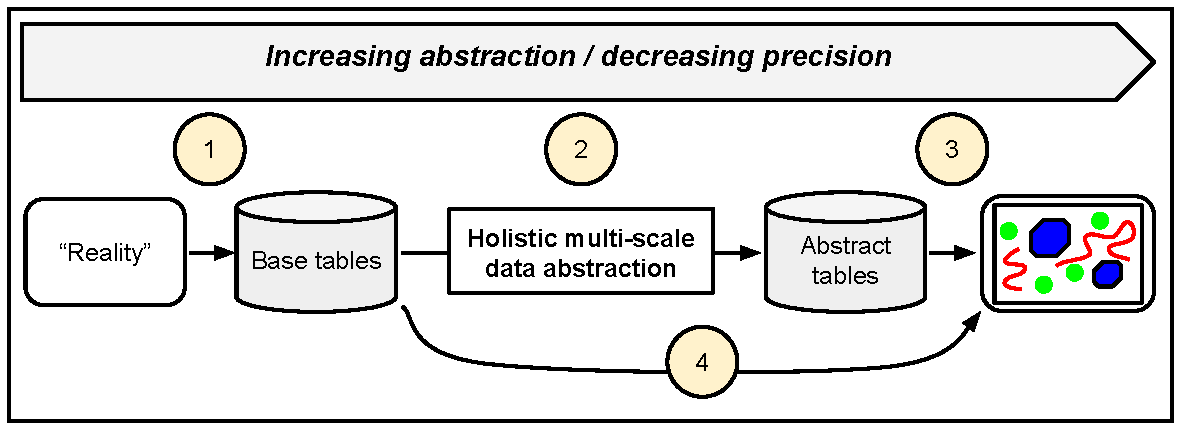
\includegraphics[scale=.6]{figs-thesis/holistic-abstraction-pipeline.pdf}
\caption{A multi-scale data visualization can abstract ``reality'' into visual representation using different paths. The path $\lbrack1,4 \rbrack$ defers all data abstraction to the visual renderer, while the path $\lbrack 1,2,3 \rbrack$ computes a multi-scale data abstraction, which is then accessed by the visual renderer. This figure is modified after Grunreich~\cite{gruenreich1985cag}}
\label{fig:related:work:data:abstraction}
\end{center}
%\vspace*{-4ex}
\end{figure}

To realize further the potential of data visualization, this thesis proposes to bring data abstraction techniques to where the data is frequently managed, i.e. relational database systems (RDBMS). The extension of RDBMS with support for data visualization induces a new class of systems, i.e. data visualization management systems (DVMS)~\cite{wu2014case}. This thesis focuses on four problems that hinder the realization of DVMS.

\subsection{Holistic Multi-scale Selection}
Panning and zooming are powerful techniques that allows users to explore data at different focal points and levels of detail~\cite{stolte2003multiscale,woodruff2001datasplash}. However, computer screens have a finite number of visual configurations by which the data can be represented. To avoid conflicts at lower scales, the set of rows must be abstracted according to principles that ensure legibility~\cite{woodruff1998constant, topfer1966principles}.  for example by selected, aggregated and projected to increase legibility and . Failing that, symbols that visually represent the rows will become increasingly cluttered at lower scales, making it impossible for users to comprehend or interact with the data. Dispite this problem, RDBMS today do not natively support operators that can (easily) express the data abstractions needed for complex, multi-scale data visualizations~\cite{wu2014case}. A critical issue is that rows must be abstracted \emph{holistically}

For example, the selection operator only allows rows to be filtered according to a row-by-row predicate. Critically, records in a data visualization must be selected, i.e. according to global criteria such as legibility and relative importance~\cite{weibel:controls:of:generalization}. Moreover, data must sometimes be consistently selected for several levels of detail, which allows users to explore more data points by zooming in. Some important questions that must be answered are:

\begin{itemize}
\item What use cases must holistic selection cover? 
\item What are the sematics of holistic selection?
\item How should holistic selection be parameterized?
\end{itemize}


%\marcos{Not obvious that SQL is or is not the obvious? So build up the argument: Why declarative versus something else? Argue for declarative (leave minute detail to a system, not to the user. Constructive approach is too time consuming). SQL already exists in databases. Argue that ideal to extend SQL.}

\todo{Reuse arguments from related work section in The Case for Visualization Management Systems~\cite{wu2014case}: % http://www.vldb.org/pvldb/vol7/p903-wu.pdf
\begin{itemize}
\item Previous work in visualization systems have traded-off between expressiveness and performance.
\item D3, protovis, and matplotlib are highly expressive, however they require low-level programming that impedes the ability to quickly iterate and do not scale to large datasets.
\item Declarative grammar-based languages, such as the Grammar of Graphics, and ggplot2 are expressive domain-specific languages designed for rapid iteration, however they do not scale beyond their host environments of SPSS and R.
\item Recent systems address these scalability limitations int two ways
\item First, by either adopting specific data management techniques such as pre-computation (Real-time visual querying of big data),  indexing (Nanocubes for real-time exploration of spatiotemporal datasets), sampling (Blinkdb: queries with bounded errors and bounded response times on very large data), speculation (Distributed and Interactive Cube Exploration), and aggregation (Dynamic reduction of query result sets for interactive visualization, Bin-summarise-smooth: a framework for visualising large data).
\item Second, by developing two-tiered architectures where the visualization client composes and sends queries to a data management backend (Polaris: A system for query, analysis and visualization of multi-dimensional relational databases, Visreduce: Fast and responsive incremental information visualization of large datasets.)
\item The former approaches are optimized towards properties of specific applications or visualization types and may not be broadly applicable.
\item The former approaches are optimized towards properties of specific applications or visualization types and may not be broadly applicable.
\end{itemize}
Managing Data for Visual Analytics: Opportunities and Challenges~\cite{fekete2012dmvis}: % https://hal.archives-ouvertes.fr/file/index/docid/272779/filename/VAChapter_final.pdf
\begin{itemize}
\item Foo
\end{itemize}
}

\subsection{Declarative Specification} 
Designers of visualizations must be able to control the selection of data. While, data abstraction can be expressed in all programming languages, it is generally not easy or time-efficient to specify a holistic selection using imperative commands. A declarative approach, which leaves the minute details to the system, and lets the user focus on higher-level goals, is arguably better. The same type of argument has been made for SQL, which is one of the most successful programming languages for selecting relational data. However, SQL and its corresponding query engines do not support holistic selection. So, for data visualization purposes, SQL must be extended with new syntax for expressing holistic selection. An important questions is:

\begin{itemize}
\item How can SQL be extended to allow designers to express holistic selection?
\end{itemize}

\todo{Reuse arguments from: The Case for Visualization Management Systems~\cite{wu2014case}: % http://www.vldb.org/pvldb/vol7/p903-wu.pdf
\begin{itemize}
\item Foo
\end{itemize}
Managing Data for Visual Analytics: Opportunities and Challenges~\cite{fekete2012dmvis}: % https://hal.archives-ouvertes.fr/file/index/docid/272779/filename/VAChapter_final.pdf
\begin{itemize}
\item Foo
\end{itemize}
}

\subsection{Scalable Data Processing} 
A query executing engine for holistic selection queries must be scalable, because the data may be large. One approach is to translate holistic selection queries to low-level code (e.g. LLVM, C++, OpenMP, or MPI), which can potentially result in very efficient execution. However, low-level code is harder to optimize across platforms. A better approach is to target a higher-level language such as SQL, which reuses optimization techniques that are built-in to SQL query engines~\cite{boncz2005pathfinder, boncz2006monetdb, grust2009ferry}. Additionally, data that underlies a visualization is frequently stored and managed in RDBMS to begin with~\cite{wu2014case}. Therefore, it makes sense to compute holistic selection on top of or inside an RDBMS, e.g. using a translation to pure SQL. Assuming that holistic selection is implemented on top of an RDBMS, some key questions are: 

\begin{itemize}
\item How can holistic selection queries be translated into scalable and efficient queries in pure SQL? 
\item How can the built-in optimizations of relational database engines be leveraged?
\end{itemize}

\subsection{Predictive Data Materialization}

\note{Mention something about the cost of CDN}

Digital maps are a type of visualization of geographical maps. Raw spatial data is transformed into a visual abstraction, the actual map. The transformation data objects to images is relatively CPU and I/O intensive. In a scalable service, we want to materialize and cache the visual abstraction ahead of time as much as possible. In order not to waste CPU and I/O resources, we want to prioritize the materialization of the map by the propabilty that parts of the map are accessed. Most web services today experience highs and lows in the number of concurrent users. If we can predict the content that will be requested during a high load window, we can exploit low-load windows perform pre-materialization. The questions that arise are:
\begin{itemize}
\item How can the prediction process be guided, e.g. by logging data?
\item How can we design a prediction model that works well for geospatial workloads?
\end{itemize}